%Este trabalho está licenciado sob a Licença Creative Commons Atribuição-CompartilhaIgual 3.0 Não Adaptada. Para ver uma cópia desta licença, visite http://creativecommons.org/licenses/by-sa/3.0/ ou envie uma carta para Creative Commons, PO Box 1866, Mountain View, CA 94042, USA.

%%%%%%%%%% PREAMBLE %%%%%%%%%%%%%%%

%%%%% language settings %%%%
\usepackage[brazil]{babel}
\usepackage[utf8]{inputenc}
\usepackage[T1]{fontenc}
%\usepackage{xunicode} é o pacote necessário para a codificação UTF-8 no XeTeX

%%%% independent chapters %%%%
\usepackage{subfiles}

%%%%% geometry %%%%%
%\usepackage[hmargin=2.5cm,vmargin=2.5cm]{geometry}

%%%% ams-latex %%%%
\usepackage{amsmath}
\usepackage{amssymb}
\usepackage{amsthm}

%%%% graphics %%%%
\usepackage{graphics}
\usepackage{graphicx}

%%%% links %%%%
\usepackage[hidelinks]{hyperref}

%%%% copy and paste from PDF (correctly) %%%%
\usepackage{upquote}
\usepackage{lmodern}

%%%% code insert (verbatim) %%%%
\usepackage{verbatim}

%%%% indent first line %%%%
\usepackage{indentfirst}

%%%% comma as a decimal separator %%%%
\usepackage{icomma}

%%%% citation %%%%
\usepackage{cite}

%%%% miscellaneous %%%%
\usepackage{multicol}
\usepackage{multirow}
\usepackage[normalem]{ulem}
\renewcommand{\arraystretch}{1.5} %space between rows in tables

%%%%%%%%%%%%%%%%%%%%%%%%%%%%%%%
%%%% Exercises and Answers %%%%
\usepackage[answerdelayed,lastexercise]{exercise}
\usepackage{chngcntr}
\counterwithin{Exercise}{section}
\counterwithin{Answer}{section}
\renewcommand{\ExerciseHeaderTitle}{({\it \ExerciseTitle})}
\renewcommand{\ExerciseName}{E}
\renewcommand{\ExerciseHeader}{{\textbf{\large\ExerciseName~\ExerciseHeaderNB\ExerciseHeaderTitle\ExerciseHeaderOrigin\medskip}}}
\renewcommand{\ExerciseHeader}{\textbf{\ExerciseName\ \ExerciseHeaderNB.}\,}

% change font for answers header
\renewcommand{\AnswerHeader}{\tiny\textbf{\ExerciseName\ \ExerciseHeaderNB.}\smallskip}
% change font for answers list header
\renewcommand{\AnswerListHeader}{{\tiny\textbf{\AnswerListName\
(\ExerciseListName\ \ExerciseHeaderNB)\ ---\ }}}
%%%%%%%%%%%%%%%%%%%%%%%%%%%%%%

%%% environments %%%%
\theoremstyle{plain}          %   bold title, italic body
\newtheorem{teo}{Teorema}[section]
\newtheorem{lem}{Lema}[section]
\newtheorem{prop}{Proposição}[section]
\newtheorem{corol}{Corolário}[section]
\newtheorem{defn}{Definição}[section]
\theoremstyle{remark}           % italic title, romman body
\newtheorem{obs}{Observação}[section]
\theoremstyle{definition}       % italic title, romman body
\newtheorem{ex}{Exemplo}[section]


\newenvironment{sol}
{\let\oldqedsymbol=\qedsymbol
  \renewcommand{\qedsymbol}{$\Diamond$}
  \begin{proof}[\bfseries\upshape Solução]}
  {\end{proof}
  \renewcommand{\qedsymbol}{\oldqedsymbol}}

%%%% newcommands %%%%
\newcommand{\sen}{\operatorname{sen}\,}
\newcommand{\tg}{\operatorname{tg}\,}
\newcommand{\p}{\partial}

%%%% page layout %%%%
\usepackage{fancyhdr}
\pagestyle{fancyplain}
\lhead[\fancyplain{}{\em\thepage}]%
  {\fancyplain{}{\em\rightmark}}
\rhead[C\'{a}lculo Num\' erico]%
  {\fancyplain{}{\em\thepage}}
%license footnote
\cfoot{\tiny{Licença CC-BY-SA-3.0. Contato: \url{livro_colaborativo@googlegroups.com}}}

%%%% no blank pages between chapters %%%%
\let\cleardoublepage\clearpage

%emphasis \emph
\DeclareTextFontCommand{\emph}{\bfseries}

%%%% indexing %%%%
\usepackage{makeidx}
\makeindex

\usepackage{xcolor}
\newcommand{\RED}[1]{{\color{red}{#1}}}
\newcommand{\BLU}[1]{{\color{blue}{#1}}}
\newcommand{\GRE}[1]{{\color{darkgreen}{#1}}}


%%%% COMPUTATION CODES %%%%
%%%% scilab?
\newif\ifisscilab
\isscilabtrue
%\isscilabfalse

%%%% octave?
\newif\ifisoctave
%\isoctavetrue
\isoctavefalse

%%%% titlepage figure %%%%
\usepackage{eso-pic}
\newcommand\BackgroundPic{%
\put(0,0){%
\parbox[b][\paperheight]{\paperwidth}{%
\vfill
\centering
\includegraphics[width=\paperwidth,height=\paperheight,%
keepaspectratio]{./rosto/capa.eps}%
\vfill
}}}
